\title{Grundlagen und Stand der Forschung}
\author{
Konstantin Tkachuk
}
\date{\today}

\documentclass[12pt]{article}
\usepackage[utf8]{inputenc}
\usepackage[T1]{fontenc}
\usepackage{lmodern}
\usepackage[ngerman]{babel}
\usepackage{graphicx}
\usepackage{url}
\usepackage{parskip}


\begin{document}
\maketitle


\section{Grundlagen}
In diesem Kapitel werden die für diese Arbeit relevanten Grundlagen erläutert, sowie der aktuelle Stand der Forschung vorgestellt.

\subsection{Internet of Things}
Die enorm steigende Anzahl von „intelligenten Gegenständen“ mit eingebetteten Computern, die den Menschen im alltäglichen Leben unterstützen sollen, hat zu der Prägung des Begriffs „Internet der Dinge“ (IoT) geführt. Jedes dieser Dinge hat seine eigene Funktionalität und im Verbund stellen sie eine große Menge an Daten zur Verfügung. Im Rahmen von zahlreichen Forschungsprojekten \cite{ierc:portfolios} werden Möglichkeiten untersucht, IoT mit unterschiedlichen Technologien zu kombinieren. Unter anderem werden Technologien, wie Cloud Computing, Machine-2-Machine Learning und Semantic Web untersucht. Außerdem werden Kernprinzipien, wie Architektur und Standardisierung intensiv recherchiert. Sie werden in dedizierten Forschungsprojekten \cite{icore:achitecture}\cite{iota:d25} immer wieder aufgegriffen.

Im Laufe der Zeit haben sich verschiedene Aspekte des IoT herausgebildet, unter anderem das Smart Home.

\subsection{Smart Home}
Ein mit IoT eng verwobenes Thema ist das Smart Home, welches die elektronische Steuerung von ausgewählten Geräten mit z.B. einer Rule Engine kombiniert um eine Automatisierung des Geräteverhaltens in einem Zusammenspiel zwischen Sensorik und Aktortik zu erreichen. Smart Home grenzt sich von IoT ab indem es auf Sensoren und Aktoren spezialisiert ist, die im Kontext eines Hauses relevant sind.

Bis dato wurden zahlreiche Smart Home Lösungen von verschiedenen Anbietern entwickelt. Man kann prinzipiell zwei Arten von Lösungen unterscheiden. \textit{Proprietäre} Produkte (z.B. RWE SmartHome) spezialisieren sich auf eine sehr begrenzte Anzahl von Geräten und bemühen sich maximale Unterstützung für diese Geräte zu bieten. Dies sorgt für eine Fragmentierung des Marktes. \textit{Open Source} Lösungen hingegen verfolgen das Ziel möglichst offen für verschiedene Geräte und Protokolle zu bleiben. 


\subsubsection{Eclipse SmartHome}
Eclipse SmartHome (ESH)\cite{ESH} ist Teil des Eclipse Open IoT Stacks\cite{EOIoT}. Es ist ein Framework, dass als Grundlage für die weitere Entwicklung von konkreten Smart Home Lösungen ausgelegt ist. Unter anderem kommt es in bekannten Lösungen wie openHAB und Qivicon zum Einsatz.

Eclipse SmartHome basiert auf Java OSGi, was es sehr modular macht. Es bietet allgemeine Kernfunktionalitäten, die in einem Smart Home Produkt benötigt werden. Hierzu gehören Modelle, Schnittstellen und unterstützende Services, die es Third-Party Entwicklern erleichtern eigene Bindings zu implementieren, ohne existierenden Code verändern zu müssen. Unter Binding versteht man eine implementierte Schnittstelle für ein konkretes Gerät/Service. 

Außerdem gibt es Unterstützung für die Implementierung von Discovery Services  und einer Benutzeroberfläche. Eine rudimentäre Rule Engine des Event-Condition-Action Typs, die es erlaubt das Verhalten von Geräten zu automatisieren, ist integriert. Für eine Reihe von populären Geräten (z.B. Philips Hue) sind Bindings bereits beispielhaft implementiert.

Ein Kernvorteil von ESH im Kontext dieser Arbeit ist, dass es ein Open Source Framework mit Fokus auf Offenheit ist. Diese Erweiterbarkeit des Frameworks ist von großem Interesse für die Arbeit. Mehr dazu in Sektion \ref{Ziele}.

\subsection{Task Automation Services}
Die Automatisierung von Aufgaben ist eins der zentralen Bestreben unseres alltäglichen Lebens. Es macht das Leben einfacher und erlaubt uns kostbare Zeit zu sparen. Ob Notifikation auf dem Smartphone, wenn eine Email eingeht oder das Einschalten von Lampen, wenn ein Raum betreten wird, solche Automatisierung ist heutzutage überall zu finden. Lange Zeit musste jede derartige Automatisierung einzeln entworfen, konfiguriert und implementiert werden. Doch die steigende Anzahl von intelligenten Gegenständen und die Allgegenwärtigkeit des Internets belassen dies der Vergangenheit. Nun hat sich der Ansatz der Task Automation Services\cite{ieee:tas} gebildet.

Ein Task Automation Service (TAS) ist ein Dienst, der es Endnutzern ermöglicht das Verhalten von verschiedenen Services und Geräten in eigenen Szenarien jederzeit selbst zu automatisieren. Solche Szenarien basieren auf Event-Condition-Action (ECA)\cite{ECA} Regeln, welche es ermöglichen, auf Events unter festgelegten Bedingungen mit entsprechenden Aktionen zu reagieren. Meistens wird dies durch  einen intuitiven visuellen Regel Editor ermöglicht.

%evtl näher eingehen, was typische Charakteristika von TAS sind: Channels, channel paradigms

Aktuell gibt es noch vergleichsweise wenige TAS. Ein Überblick über existierende  Services bietet Abbildung \ref{fig:tasoverview}.

%Aktuell gibt es eine Reihe von TAS in der Cloud. Sie erlauben es zahlreiche Services miteinander zu verknüpfen, und entsprechend zu reagieren. Diese Services haben den Vorteil, dass sie jederzeit von überall erreichbar sind. Allerdings haben sie auch Nachteile, vor allem was den Datenschutz betrifft.

\begin{figure}[h]
	\centering
	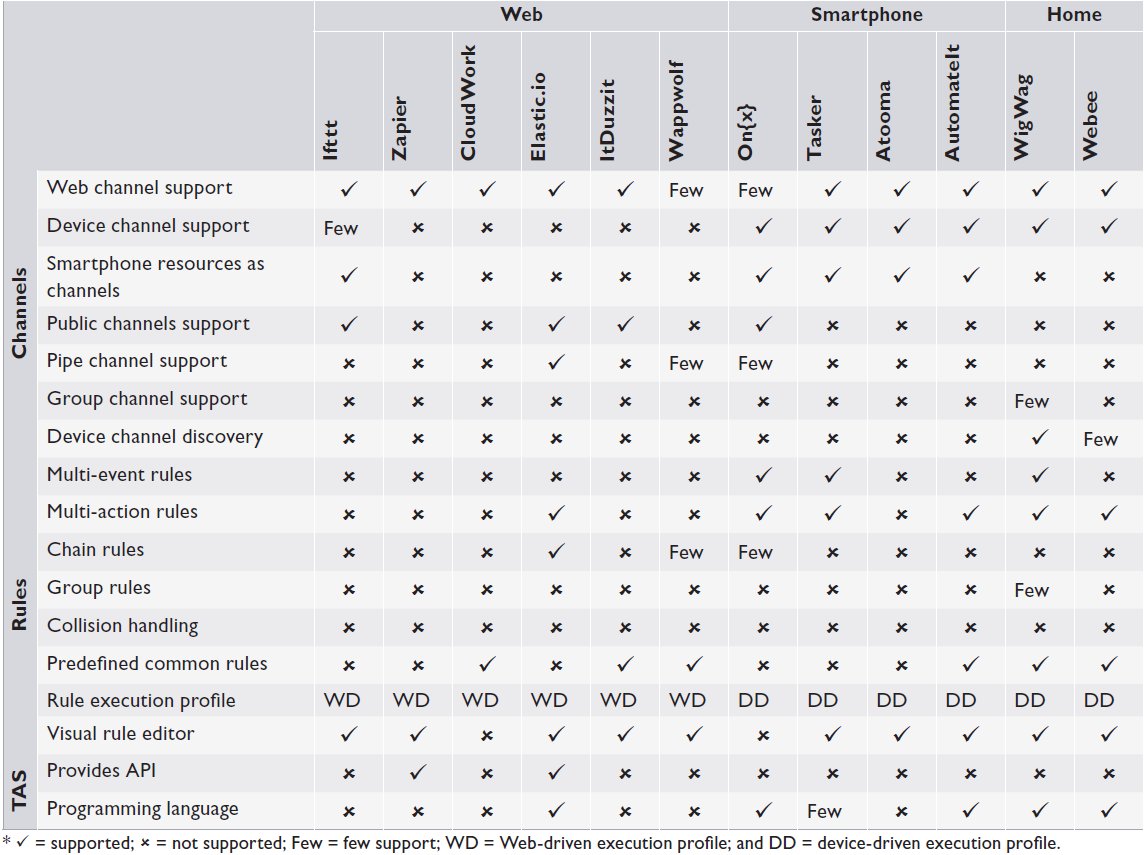
\includegraphics[width=\textwidth]{TASOverview}
	\caption{Überblick über existierende Task Automation Services \cite{ieee:tas}}
	\label{fig:tasoverview}
\end{figure}

Wie in der Abbildung zu sehen ist, gibt es unterschiedliche Ansätze. Einige TAS sind in der Cloud angesiedelt, was bedeutet, dass sie, sofern Internet verfügbar ist, jederzeit und von überall erreichbar sind. Die aktuell mächtigsten und bekanntesten TAS sind IFTTT\cite{IFTTT} und Zapier\cite{Zapier}. Sie unterstützen hunderte unterschiedlicher Web Services, bieten aber keine Möglichkeit mit Geräten direkt zu interagieren. Um diese TAS zu nutzen, muss man jedoch bereit sein, sämtliche Zugriffsdaten, die für die zu automatisierenden Dienste (z.B. Facebook, Twitter, etc.) benötigt werden, dem TAS anzuvertrauen.

Andere Task Automation Services arbeiten lokal auf Smartphones. Solche TAS konzentrieren sich auf die Automatisierung von den auf dem Gerät laufenden Services. Die Unterstützung von der Automatisierung von Web Services ist nur in dem Umfang gegeben, in dem diese Web Services direkten Kontakt mit dem Smartphone haben.

Schließlich gibt es TAS, die auf einer dedizierten Basis im Haus arbeiten. Solche Task Automation Services konzentrieren sich auf die direkte Steuerung von Geräten mithilfe der entsprechenden Protokolle. Im Grunde sind sie äquivalent zu Smart Home. 

Im Rahmen dieser Arbeit wird Smart Home jedoch getrennt von TAS behandelt, da der Fokus der Automatisierung völlig unterschiedlich ist. Mehr dazu in Sektion \ref{sdf}.

Wie zu sehen ist, unterstützen aktuelle TAS nur begrenzt die direkte Steuerung von Geräten. Außerdem sind die zum Einsatz kommenden Rule Engines sehr rudimentär. Dies ermöglicht den Endnutzern zwar leichteren Einstieg in den visuellen Regeleditor, begrenzt aber auch gleichzeitig stark ihre Mächtigkeit. 



%\subsubsection{IFTTT}
%Ein Beispiel für Task Automation Services in der Cloud ist IFTTT, welches eine große Anzahl verschiedener Services (\textit{Facebook}, \textit{Philips Hue}, \textit{Dropbox}, etc.) integriert und eine rudimentäre Rule Engine anbietet, die es erlaubt auf eine einfache Art und Weise serviceübergreifende „if this than that“ Anweisungen zu hinterlegen, die der klassischen „EDV“ ähneln. Es wird eine feste Trigger Komponente gewählt, die etwas auslöst, daraufhin wird die Aktion festgelegt, die ausgeführt werden soll. Solche Condition/Command Paare werden in IFTTT Recipes genannt. 

%Bis dato lassen sich komplexere Szenarien mit \textit{IFTTT} nicht abbilden.  Das bedeutet, dass es keine Möglichkeit gibt, beispielsweise, Und- und Oder-Bedingungen zu definieren, die es ermöglichen würden, mehrere Conditions in einem Recipe zu verknüpfen.

%Ein weiterer Aspekt von IFTTT ist, dass es für die Anbindung von Services der entsprechenden Passwörter des Users bedarf. Aus einer Datenschutz-Perspektive stellt das ein Risiko für den Endnutzer dar, da seine sämtlichen Account-Daten an einer Stelle gesammelt sind. Im Falle einer Sicherheitslücke bei IFTTT wären alle damit gekoppelten Services in Gefahr. 





\subsection{Vision}
\label{Vision}
In dieser Sektion werden der Stand der Forschung nochmals zusammengefasst und daraus die konkreten Ziele der Arbeit abgeleitet.

\subsubsection{Stand der Forschung}
\label{sdf}
Wie in den vorherigen Sektionen zu sehen ist, haben Smart Home und Task Automation Services viel gemeinsam. Sowohl Smart Home als auch TAS beschäftigen sich mit der Automatisierung des Verhaltens von Geräten und Services. In beiden Fällen kommen Event-Condition-Action Regeln zum Einsatz. In beiden Umgebungen spielen intuitive visuelle Regeleditoren eine wichtige Rolle. Der wesentliche Unterschied besteht lediglich in dem Fokus der Automatisierung.

Smart Home konzentriert sich auf die direkte Kommunikation mit Geräten über die entsprechenden Protokolle. Es arbeitet in der Regel on-premise und bietet die Automatisierung der Geräte. Webbasierte TAS hingegen sind auf die Automatisierung der Interaktionen zwischen Services spezialisiert.

Webbasierte TAS haben zwei wesentliche Nachteile, die auf ihre Natur zurückzuführen sind. Erstens, dadurch, dass sie in der Cloud angesiedelt sind, lässt sich keine direkte Kommunikation mit Geräten (wie in Smart Home) umsetzen. Steuerung von konkreten Geräten ist nur in dem Umfang möglich, in dem zugehörige Hersteller eine entsprechende webbasierte Schnittstelle anbieten. Intelligente Geräte ohne solche Schnittstellen lassen sich gar nicht steuern. Außerdem würde bei einem Verbindungsausfall die gesamte Gerätesteuerung ausfallen.

Zweitens, das Problem des Datenschutzes. Um die Kontrolle für den Endnutzer zu übernehmen braucht das TAS Zugriffsdaten auf die entsprechenden Services. Dies führt dazu, dass sämtliche Accounts des Nutzers \textit{an einem Ort} bei dem TAS Anbieter gelagert sind. Dies stellt ein enormes Sicherheitsrisiko dar, da   die Daten auf einem dem Nutzer unbekannten Server gelagert sind, auf den Unberechtigte sich Zugriff verschaffen können. Im Falle eines solchen Zugriffs würden die Daten des Nutzers nicht nur für \textit{einen} Service gestohlen, sondern für \textit{alle} mit dem TAS verbundenen Serivces.


\subsubsection{Ziele}
\label{Ziele}
Ziel dieser Arbeit ist es die Welten von Smart Home und webbasierten Task Automation Services zusammen zu bringen. Durch die Integration mit Smart Home soll die direkte Steuerung von Geräten ermöglicht werden. Außerdem soll die Mächtigkeit der Smart Home Rule Engine genutzt werden, um komplexere Szenarien zu ermöglichen. Schließlich sollen die Datenschutzprobleme gelöst werden, indem sämtliche Zugriffsdaten on-premise galagert und dadurch nie einem Risiko ausgesetzt werden.

Es soll ein Demonstrator entwickelt werden, der die Funktionalitäten von Smart Home und TAS kombiniert und in einer on-premise Anwendung anbietet. Hierzu soll das Eclipse SmartHome Framework als Basis verwendet werden und um die Funktionalitäten von web-basierten TAS angereichert werden. Die entstandene Anwendung soll auf einem Raspberry Pi laufen.

Die entstandenen Funktionalitäten sollen anhand von einer Reihe von konkreten Services demonstriert werden. Unter anderem sollen ein Wetterdienst, ein Filesharing Service und ein Social Media Service angebunden werden. Die Zusammenarbeit dieser Services untereinander und mit Smart Home Geräten soll anhand von Beispiel-Regeln demonstriert werden. Außerdem soll es möglich sein neue Regeln zum System über eine Benutzeroberfläche hinzufügen zu können.

Zum Schluss soll der entstandene Demonstrator evaluiert werden. Es soll geprüft werden, inwiefern Task Automation Services als on-premise Lösung sinnvoll sind unter Betrachtung von Aspekten wie Reaktionszeiten und Netzwerklast. Hierzu soll ein Vergleich der erstellten Anwendung mit IFTTT stattfinden.

%\nocite{*}

\bibliographystyle{abbrv}
\bibliography{literatur}

\end{document}

